\chapter{Основные теоретические сведения}

Изучение архитектуры суперскалярных конвейерных микропроцессоров используется синтезируемое описание микропроцессорного ядра Taiga, реализующего систему команд RV32I семейства RISC-V. Данное описание выполнено на языке описания аппаратуры SystemVerilog.

Термин RISC-V является названием для семейства различных систем команд, которые строятся вокруг базового набора команд, путем внесения в него различных расширений. В данной работе исследуется набор команд RV32I, который включает в себя основные команды 32-битной целочисленной арифметики кроме умножения и деления.

\chapter{Задание 1}

Дизассемблировать программу по индивидуальному варианту.

\section{Результат выполнения}

На рисунке \ref{img:code-asm} представлен исходный текст исследуемой программы для варианта № 18.

\begin{figure}[H]
	\begin{center}
		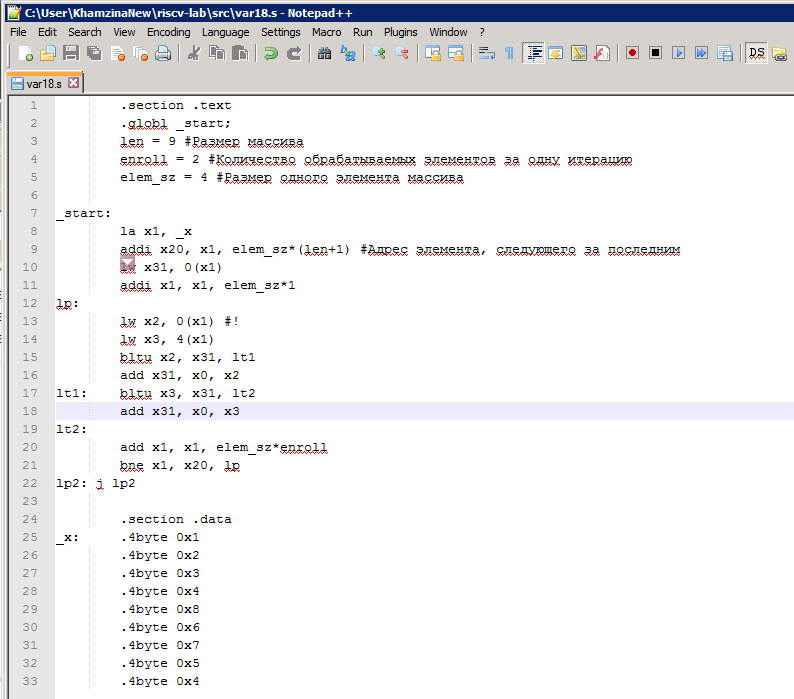
\includegraphics[scale=0.5]{img/code_asm.png}
	\end{center}
	\captionsetup{justification=centering}
	\caption{Текст программы}
	\label{img:code-asm}
\end{figure}

Дизассемблерный листинг данной программы показан на рисунке \ref{img:code-disasm}.

\begin{figure}[H]
	\begin{center}
		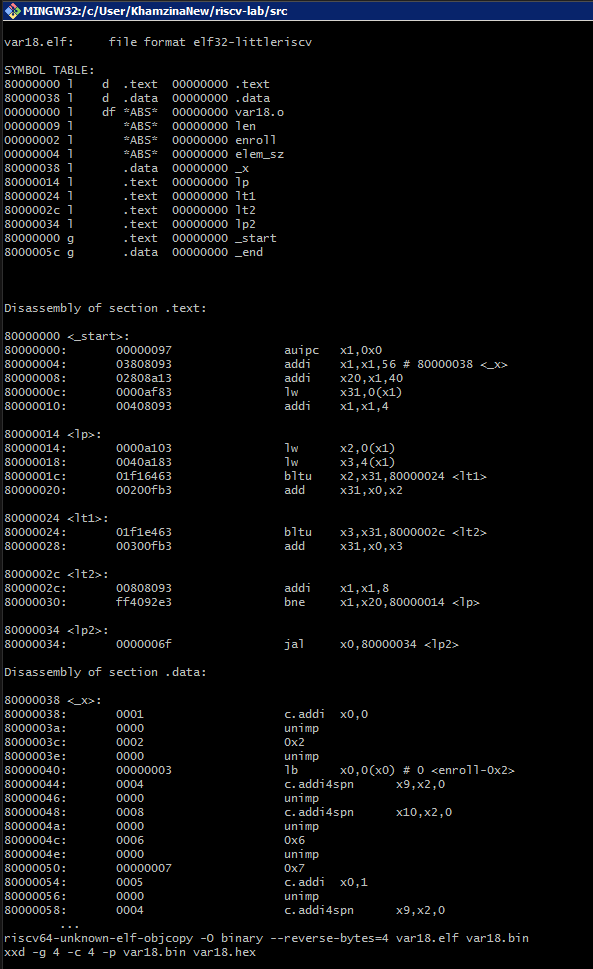
\includegraphics[scale=0.7]{img/code_disasm.png}
	\end{center}
	\captionsetup{justification=centering}
	\caption{Дизассемблированный листинг исходной программы}
	\label{img:code-disasm}
\end{figure}

В листинге \ref{lst:code} приведен псевдокод на языке C, поясняющий работу представленной программы.

\begin{center}
\captionsetup{justification=raggedright,singlelinecheck=off}
\begin{lstlisting}[label=lst:code,caption=Псевдокод программы на языке C]
#define LEN 9
#define ENROLL 2
#define ELEM_SZ 4

int _x[] = {1, 2, 3, 4, 8, 6, 7, 5, 4};

int main(void)
{
	int* x1 = _x;
	int x20 = ELEM_SZ * (LEN + 1);
	int x31 = _x[0];
	x1 += ELEM_SZ * 1
	
	do
	{
	    int x2 = x1[0];
	    int x3 = x1[4];
	    
	    if ( !(x2 < x31) )
	    {
	        x31 = x2;
	    }
	    
	    if ( !(x3 < x31) )
	    {
	        x31 = x3;
	    }
	    
	    x1 += ELEM_SZ * ENROLL;
	    
	} while ( x1 != x20 );
	
	while ( 1 ) {}
}
\end{lstlisting} 
\end{center}

\section{Вывод}

Проанализировав исходный текст программы, можно сделать вывод о том, что в регистре x31 в конце выполнения программы должно содержаться значение 0x8.

\chapter{Задание 2}

Получить снимок экрана, содержащий временную диаграмму выполнения стадий выборки и диспетчеризации команды с
адресом 8000002 на 2-ой итерации.

\section{Результат выполнения}

На рисунке \ref{img:8024} представлена диаграмма, соответствующая этапам выборки и диспетчеризации требуемой команды.

\begin{figure}[H]
	\begin{center}
		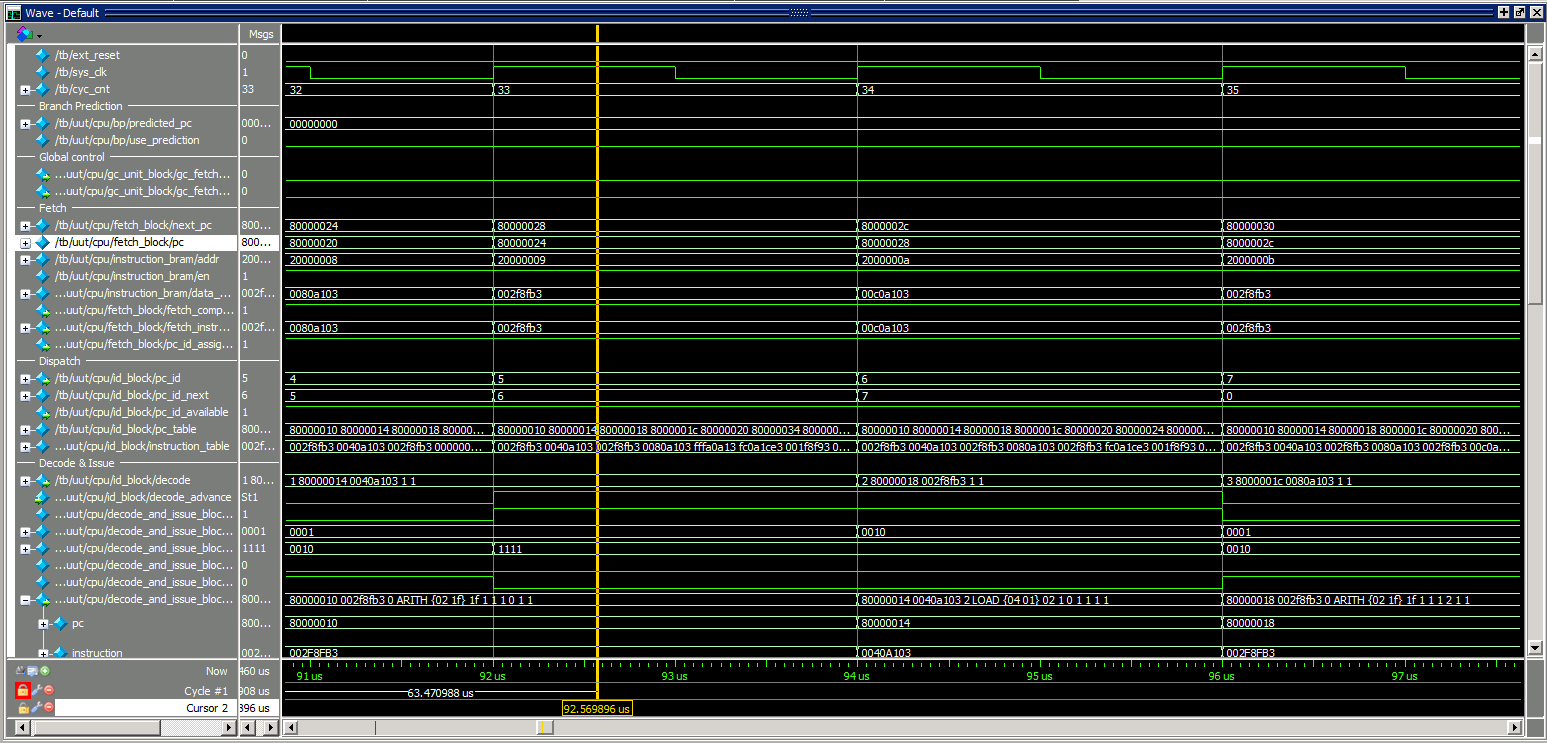
\includegraphics[scale=0.3]{img/8024.png}
	\end{center}
	\captionsetup{justification=centering}
	\caption{Диаграмма, соответствующая этапам выборки и диспетчеризации}
	\label{img:8024}
\end{figure}

\section{Вывод}

Выборка и диспетчеризация данной команды происходят на 33 и 34 тактах соответственно.

\chapter{Задание 3}

Получить снимок экрана, содержащий временную диаграмму выполнения стадии декодирования и планирования на выполнение
команды с адресом 80000030 на 2-ой итерации.

\section{Результат выполнения}

Диаграмма, соответствующая этапам декодирования и
планирования требуемой команды, показана на рисунке \ref{img:8030}.

\begin{figure}[H]
	\begin{center}
		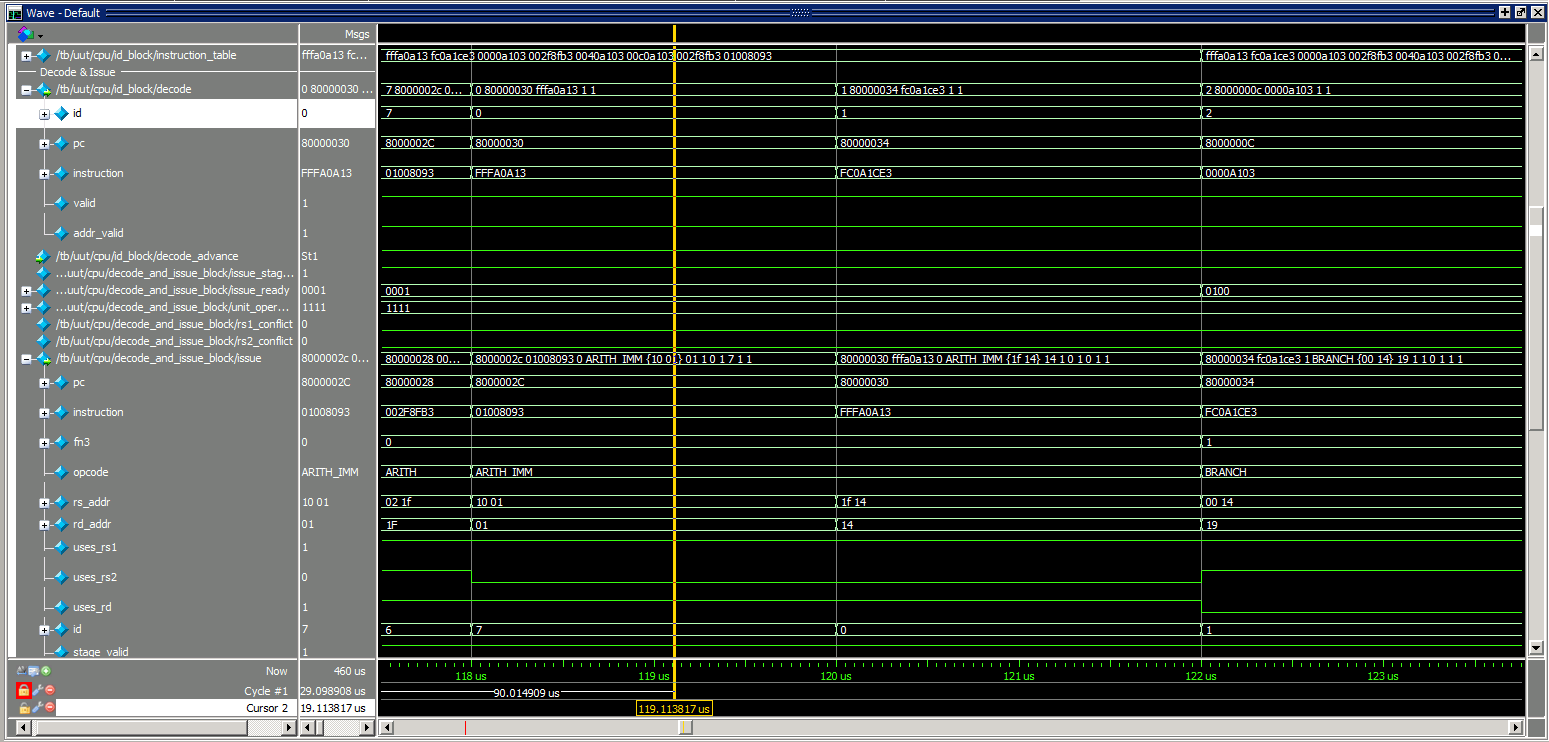
\includegraphics[scale=0.3]{img/8030.png}
	\end{center}
	\captionsetup{justification=centering}
	\caption{Диаграмма, соответствующая этапам декодирования и
планирования}
	\label{img:8030}
\end{figure}

\section{Вывод}

Так как данная команда выполняет арифметическую операцию, значения сигналов rs1\_conflict и rs2\_conflict равны 0, конфликт не возникает.

\chapter{Задание 4}

Получить снимок экрана, содержащий временную диаграмму выполнения стадии выполнения команды с адресом 8000001с на 2-ой итерации.

\section{Результат выполнения}

На рисунке \ref{img:801C} представлена диаграмма, соответствующая этапу выполнения требуемой команды.

\begin{figure}[H]
	\begin{center}
		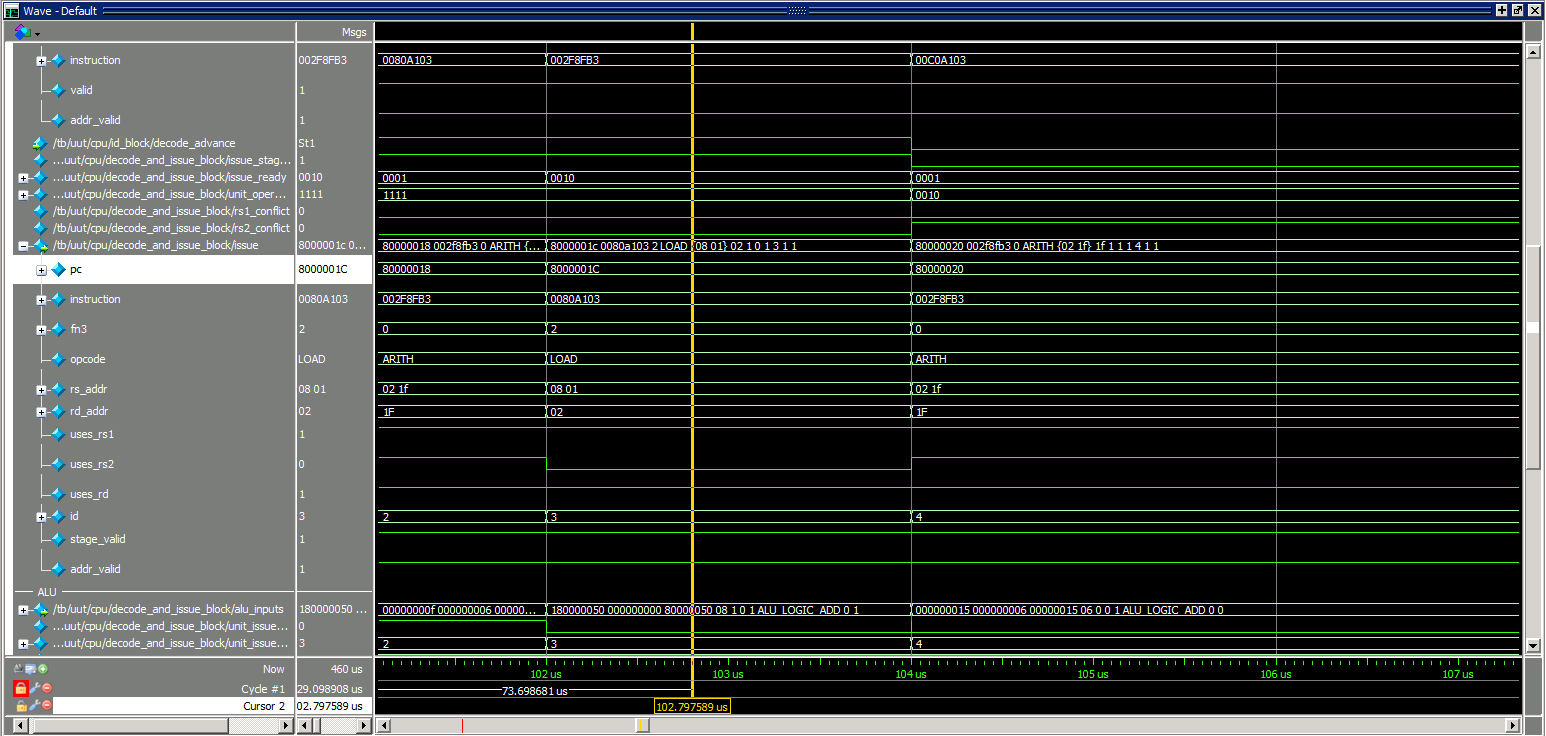
\includegraphics[scale=0.3]{img/801C.png}
	\end{center}
	\captionsetup{justification=centering}
	\caption{Диаграмма, соответствующая этапу выполнения}
	\label{img:801C}
\end{figure}

\section{Вывод}

Данная команда является командой загрузки и выполняется 3 такта. В следующем такте возникает конфликт из-за обращения к памяти, в которую происходит загрузка в текущем такте.

\chapter{Задание 5}

\section{Проверка результата}

Значение регистра x31 на момент окончания выполнения программы, показанное на рисунке \ref{img:8}, равно значению, полученному в Задании 1.

\begin{figure}[H]
	\begin{center}
		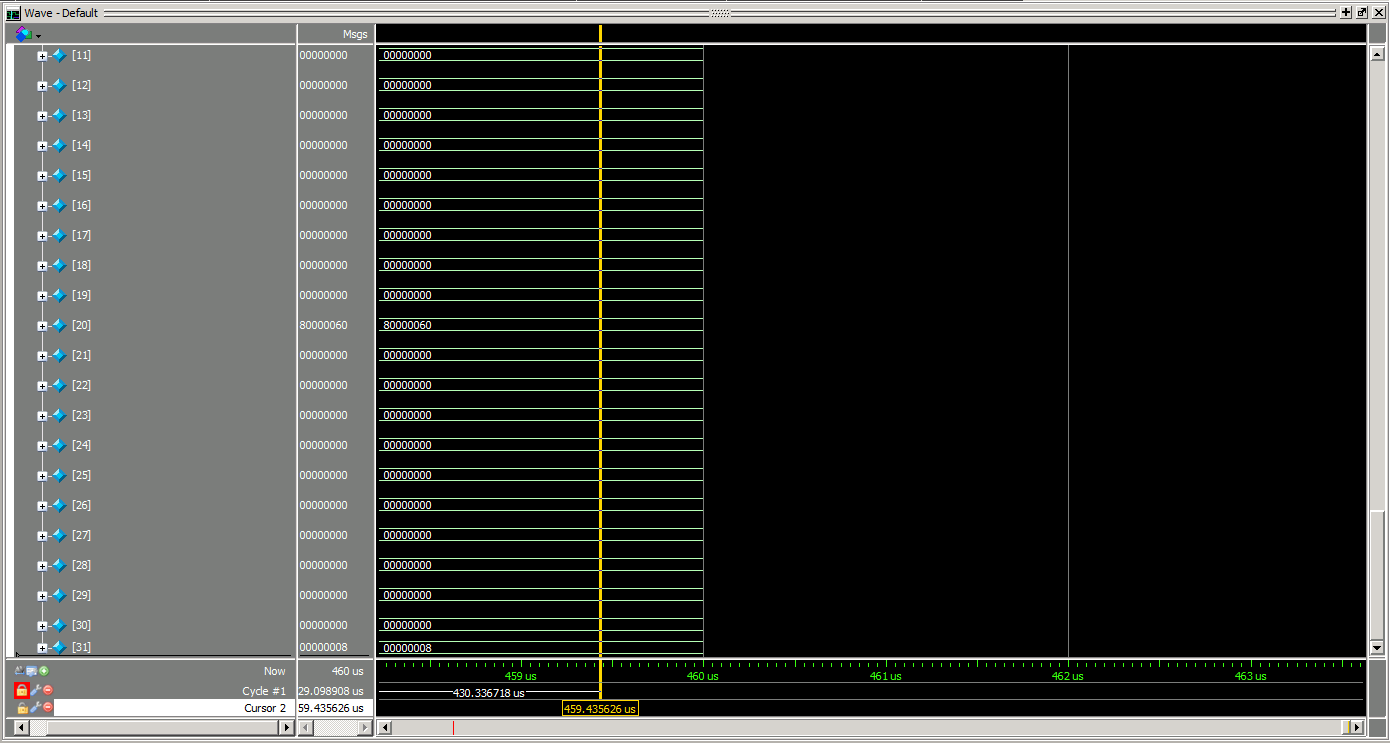
\includegraphics[scale=0.3]{img/8.png}
	\end{center}
	\captionsetup{justification=centering}
	\caption{Результат выполнения программы}
	\label{img:8}
\end{figure}

\section{Стадии выполнения команды, обозначенной в тексте программы символом}

Для программы по индивидуальному варианту № 18 заданным символом обозначена команда $lw x2,0(x1)$, находящаяся по адресу 0x80000014.

На рисунках \ref{img:cmd1}-\ref{img:cmd3} показаны временные диаграммы сигналов данной команды для стадий выборки и диспетчеризации, декодирования и планирования на выполнение и выполнения.

\begin{figure}[H]
	\begin{center}
		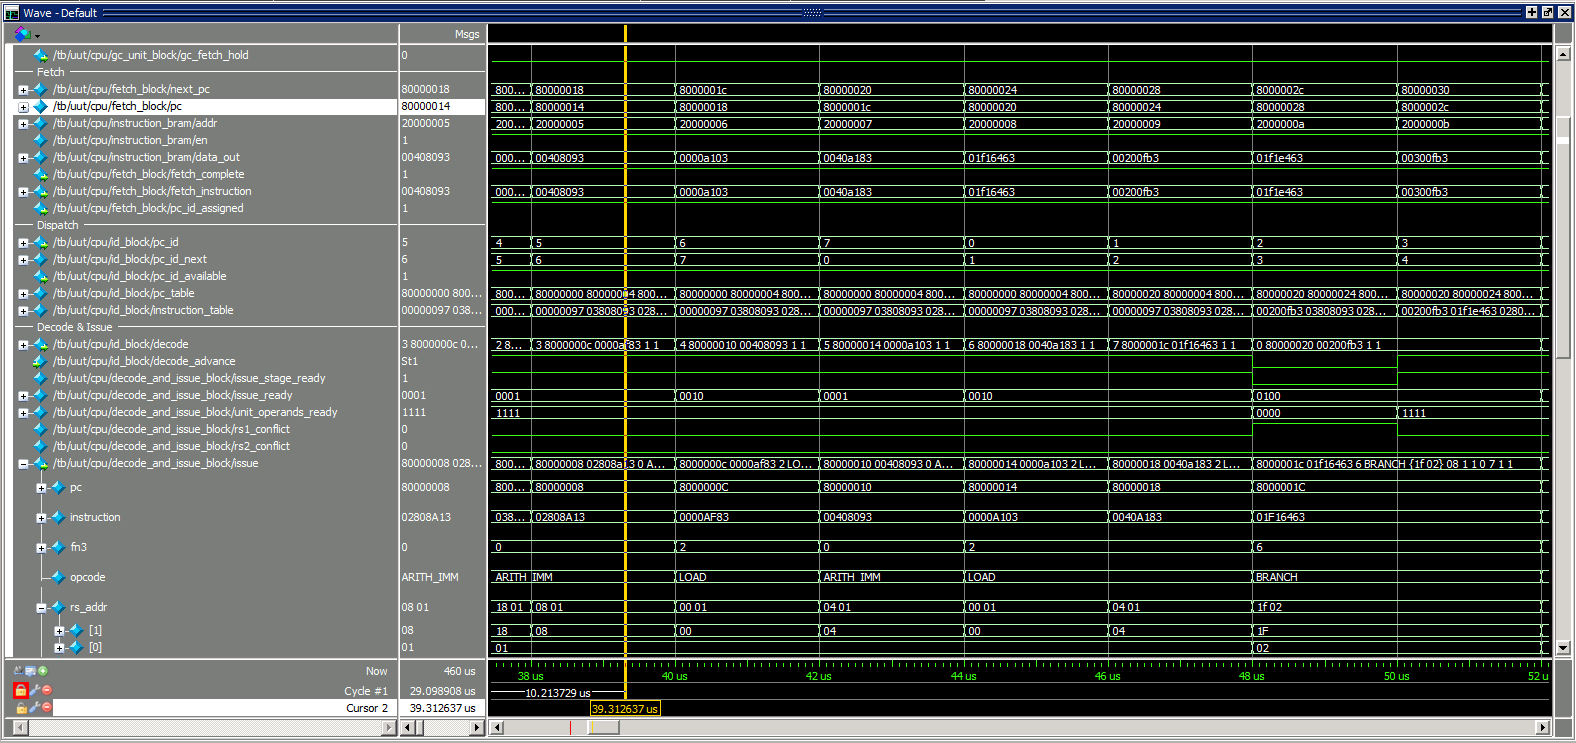
\includegraphics[scale=0.3]{img/cmd_fetch_dispetch.png}
	\end{center}
	\captionsetup{justification=centering}
	\caption{Выборка и диспетчеризация команды}
	\label{img:cmd1}
\end{figure}

\begin{figure}[H]
	\begin{center}
		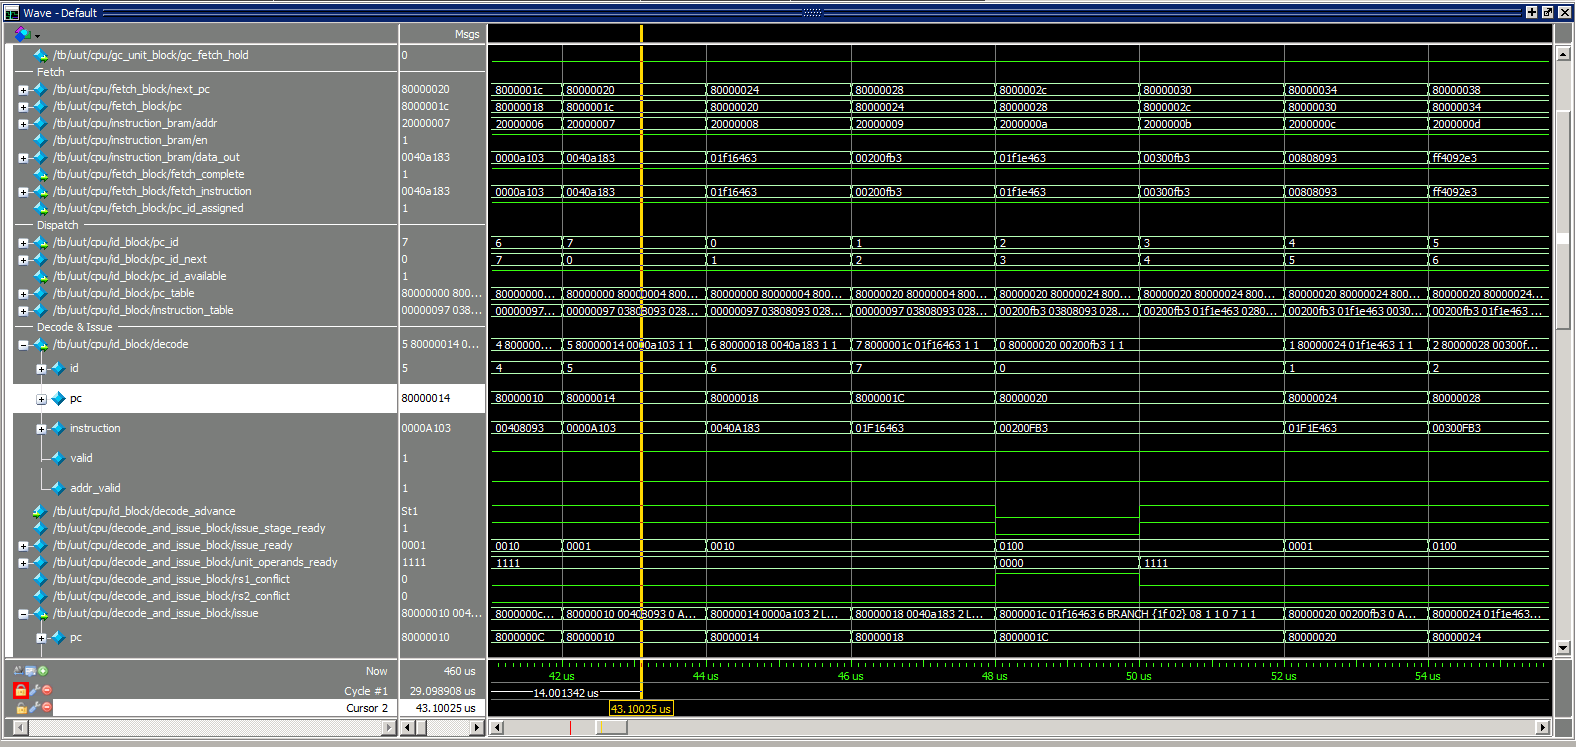
\includegraphics[scale=0.3]{img/cmd_decode.png}
	\end{center}
	\captionsetup{justification=centering}
	\caption{Декодирование команды}
	\label{img:cmd2}
\end{figure}

\begin{figure}[H]
	\begin{center}
		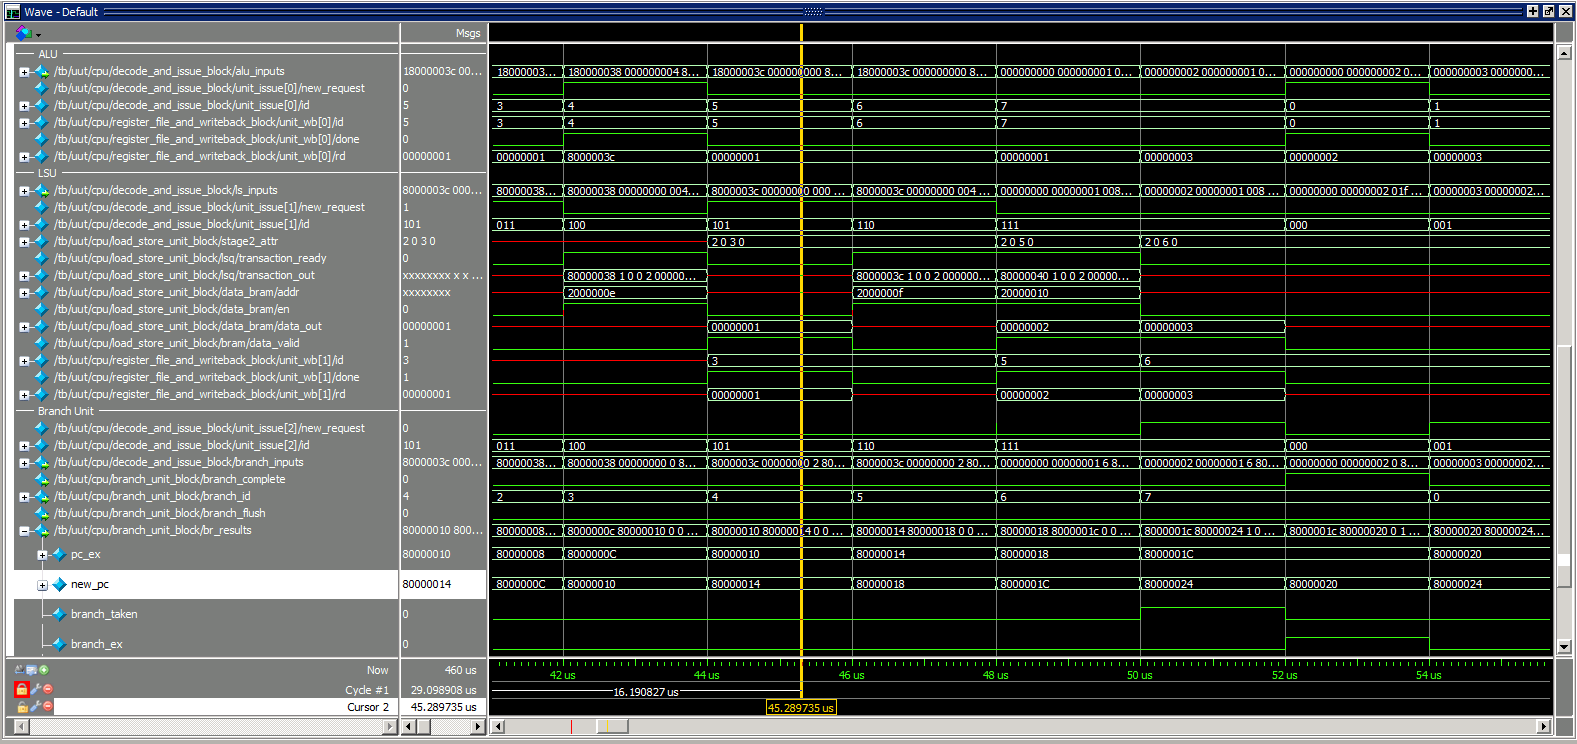
\includegraphics[scale=0.3]{img/cmd_vipoln.png}
	\end{center}
	\captionsetup{justification=centering}
	\caption{Выполнение команды}
	\label{img:cmd3}
\end{figure}

\section{Трасса выполнения программы}

Анализируя трассу выполнения программы, представленной на рисунке \ref{img:pipeline-18}, можно сделать вывод о том, что конфликты возникают тогда, когда блок обращения к памяти не
успевает загрузить необходимое для выполнения команды условного перехода ($bltu x2,x31$) значение. Это происходит потому, что блок обращения к памяти выполняет загрузку за три такта, а команда условного перехода следует за загрузкой нужной переменной через одну команду, таким образом блок обращения к памяти только завершает третий такт обработки.

\begin{figure}[H]
	\begin{center}
		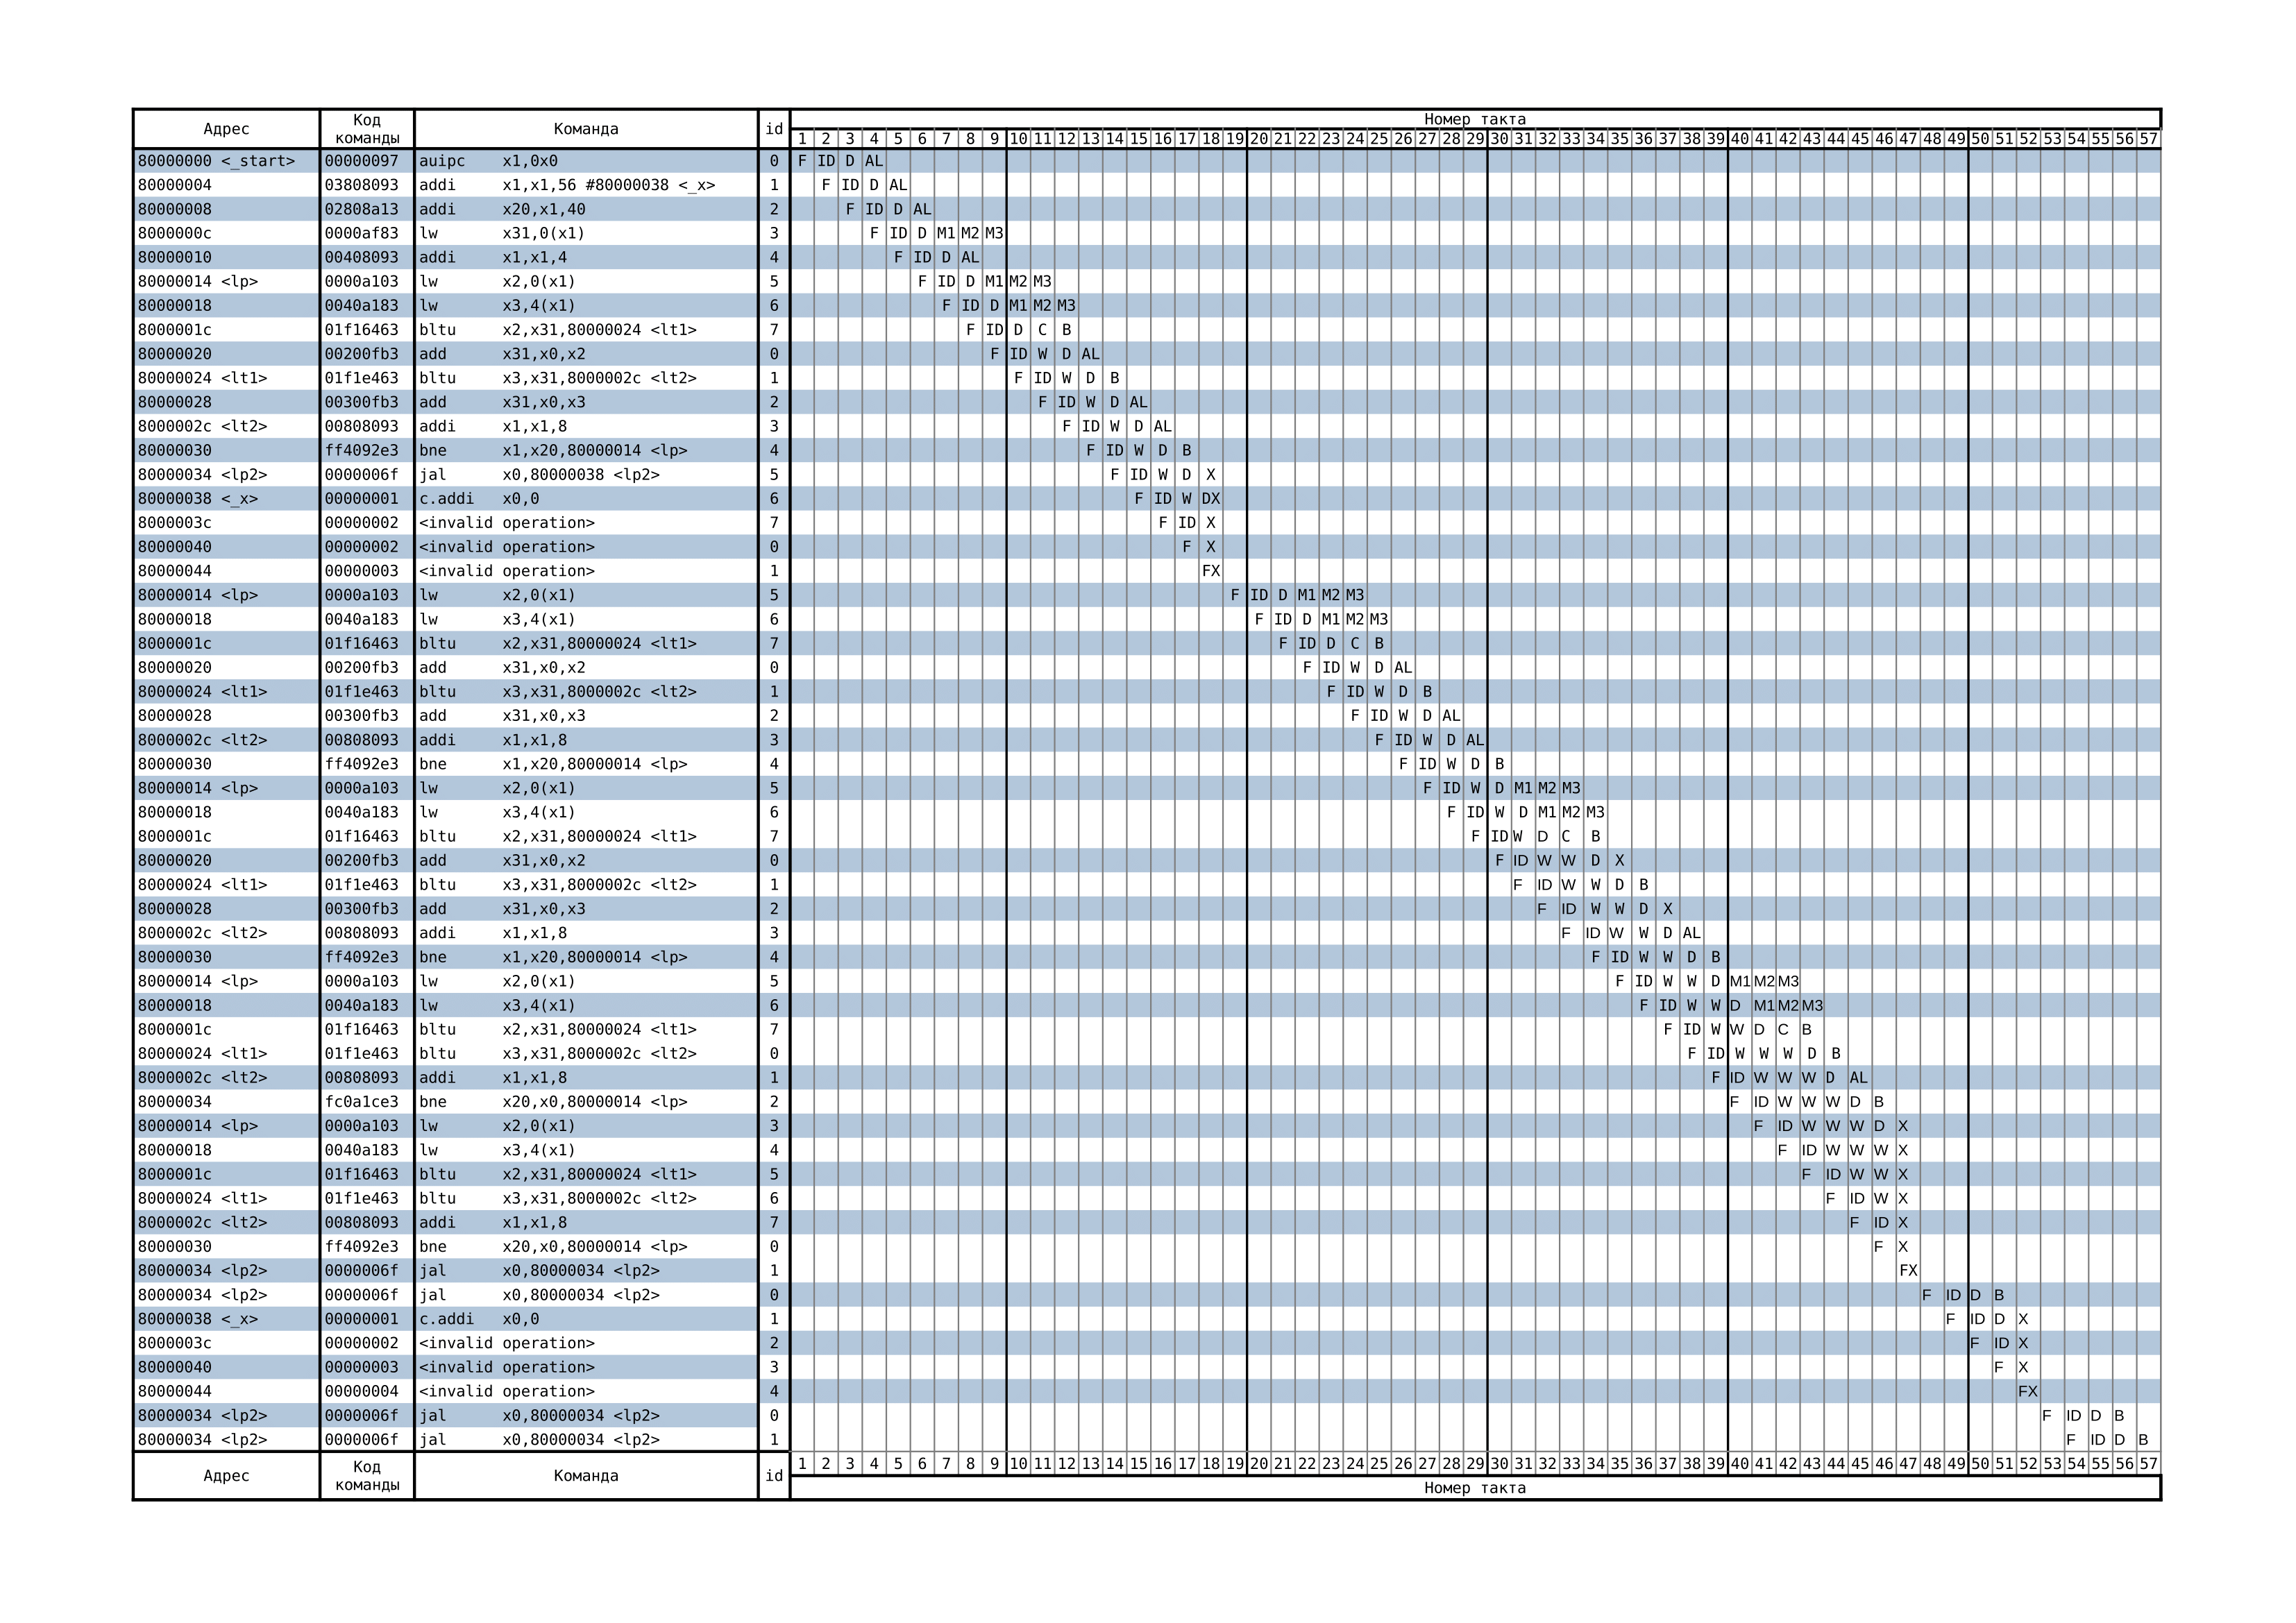
\includegraphics[scale=0.4]{img/pipeline_18.png}
	\end{center}
	\captionsetup{justification=centering}
	\caption{Трасса выполнения программы}
	\label{img:pipeline-18}
\end{figure}

\section{Оптимизация программы}

Для оптимизации программы необходимо переставить команды для устранения конфликтов: число конфликтов можно сократить, если вынести команды загрузки значений x2 и x3 из цикла, в таком случае конфликт возникнет только при первой итерации цикла.

На рисунке \ref{img:fixed} приведен текст оптимизированной программы по индивидуальному варианту, на рисунке  \ref{img:fixed-dis} - ее дизассемблерный листинг.

\begin{figure}[H]
	\begin{center}
		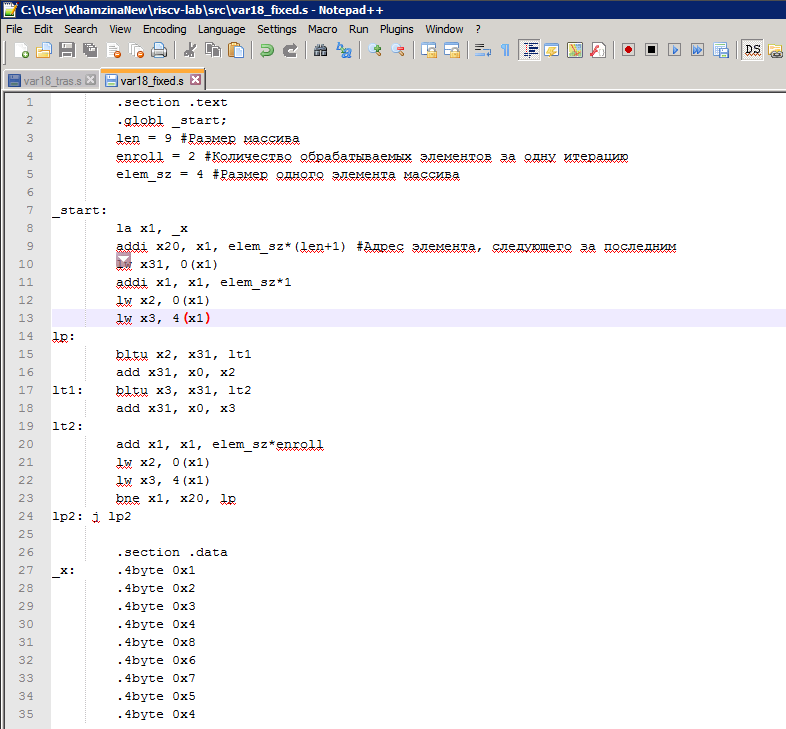
\includegraphics[scale=0.4]{img/code_asm_fixed.png}
	\end{center}
	\captionsetup{justification=centering}
	\caption{Оптимизированный код программы}
	\label{img:fixed}
\end{figure}

\begin{figure}[H]
	\begin{center}
		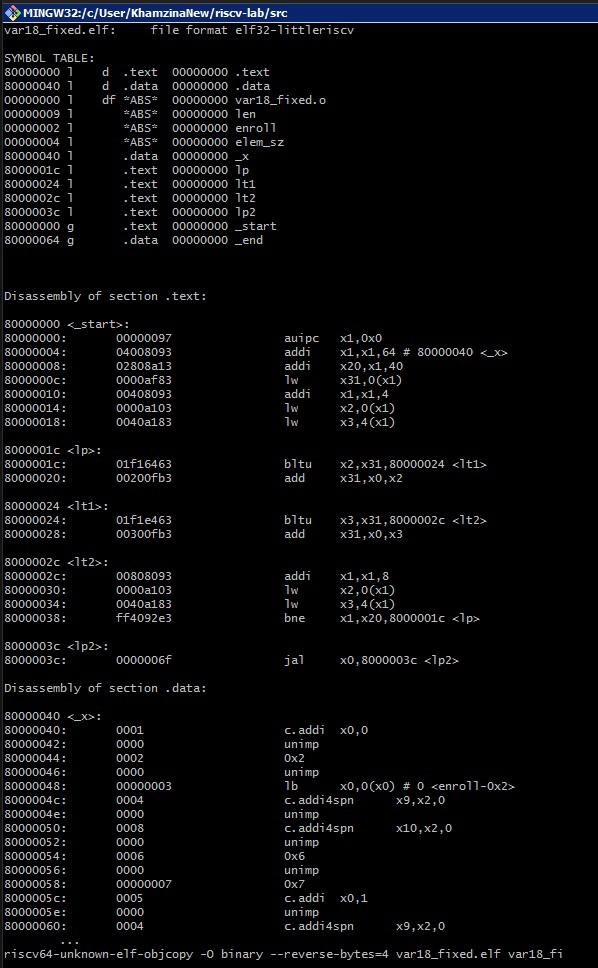
\includegraphics[scale=0.4]{img/fixed-dis.jpg}
	\end{center}
	\captionsetup{justification=centering}
	\caption{Дизассемблерный листинг оптимизированной программы}
	\label{img:fixed-dis}
\end{figure}

Трасса выполнения оптимизированной программы приведена на риснуке \ref{img:pipe}.

\begin{figure}[H]
	\begin{center}
		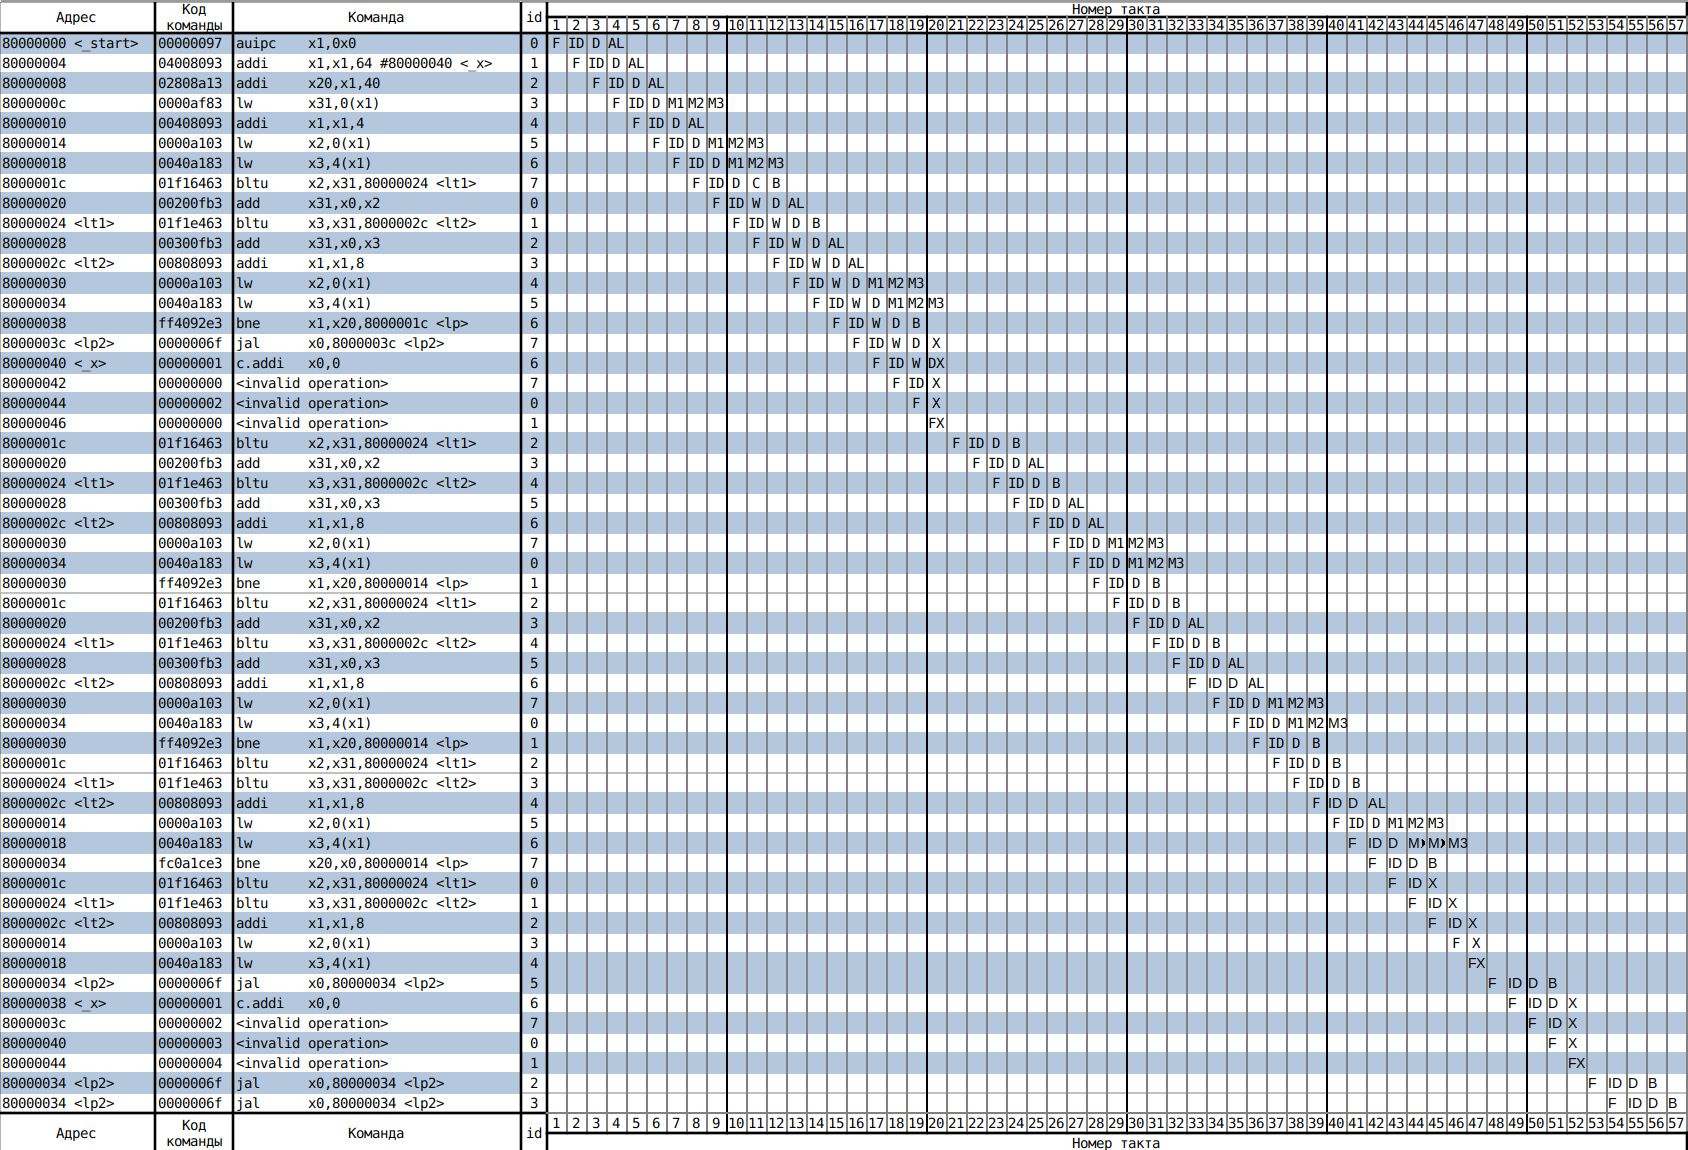
\includegraphics[scale=0.2]{img/pipe.png}
	\end{center}
	\captionsetup{justification=centering}
	\caption{Трасса выполнения оптимизированной программы}
	\label{img:pipe}
\end{figure}

В результате оптимизации удалось устранить 3 из 4 конфликтов.